\documentclass[a4paper, 12pt]{article}

\def \patha {} %Pfad zu den Dateien Preamble.tex, Commands.tex, Erwartungsbild.tex

\input{\patha/Preamble.tex}

\onehalfspacing

\newcommand{\KopfzeileBlank}{true}
\newcommand{\FACH}{Informatik}
\newcommand{\KLASSE}{5}
\newcommand{\DATUM}{XX.YY.ZZZZ}
%% Über den jeweiligen Typ wird bei Klassenarbeit und Leistungskontrolle das Erwartungsbild und der Notenspiegel als anhängende Seite kompiliert. Der Befehl \aufgabe besitzt beim Typ Arbeitsblatt einen Parameter für die Aufgabenstellung. Bei den Typen Klassenarbeit und Leistungskontrolle kommen noch zwei weitere Parameter für die Punktzahl und das Erwartungsbild hinzu.
\newcommand{\TYP}{Arbeitsblatt}
%\newcommand{\TYP}{Klassenarbeit}
%\newcommand{\TYP}{Leistungskontrolle}
\newcommand{\EINHEIT}{Bilder und Grafiken gestalten}
\newcommand{\THEMA}{Rastergrafiken}
\newcommand{\LEHRER}{}
\newcommand{\TIME}{Zeit}
\newcommand{\NTA}{Hier ist Platz für Nachteilsausgleiche!}
%% Dieser "Switch" bewirkt, dass für Lückentexte die Lösung angezeigt oder ausgeblendet wird. Aktuell werden die Lücken jedoch noch nicht berücksichtigt. Vielleicht gibt es auch eine bessere Lösung für diesen "Switch"...
%\newcommand{\LOSUNG}{true}
\newcommand{\LOSUNG}{false}

%\input
\input{\patha/Commands.tex}

\begin{document}

\large
\TITEL

\aufgabe{}
Öffne das Bild "Qualitätsraster 3x3" mit Paint.
	Nutze zur Bewerkstelligung folgender Aufgaben nur dem Fülleimer und dem Farbwähler.\\

	\begin{minipage}{0.6\textwidth}\vspace{0pt}
		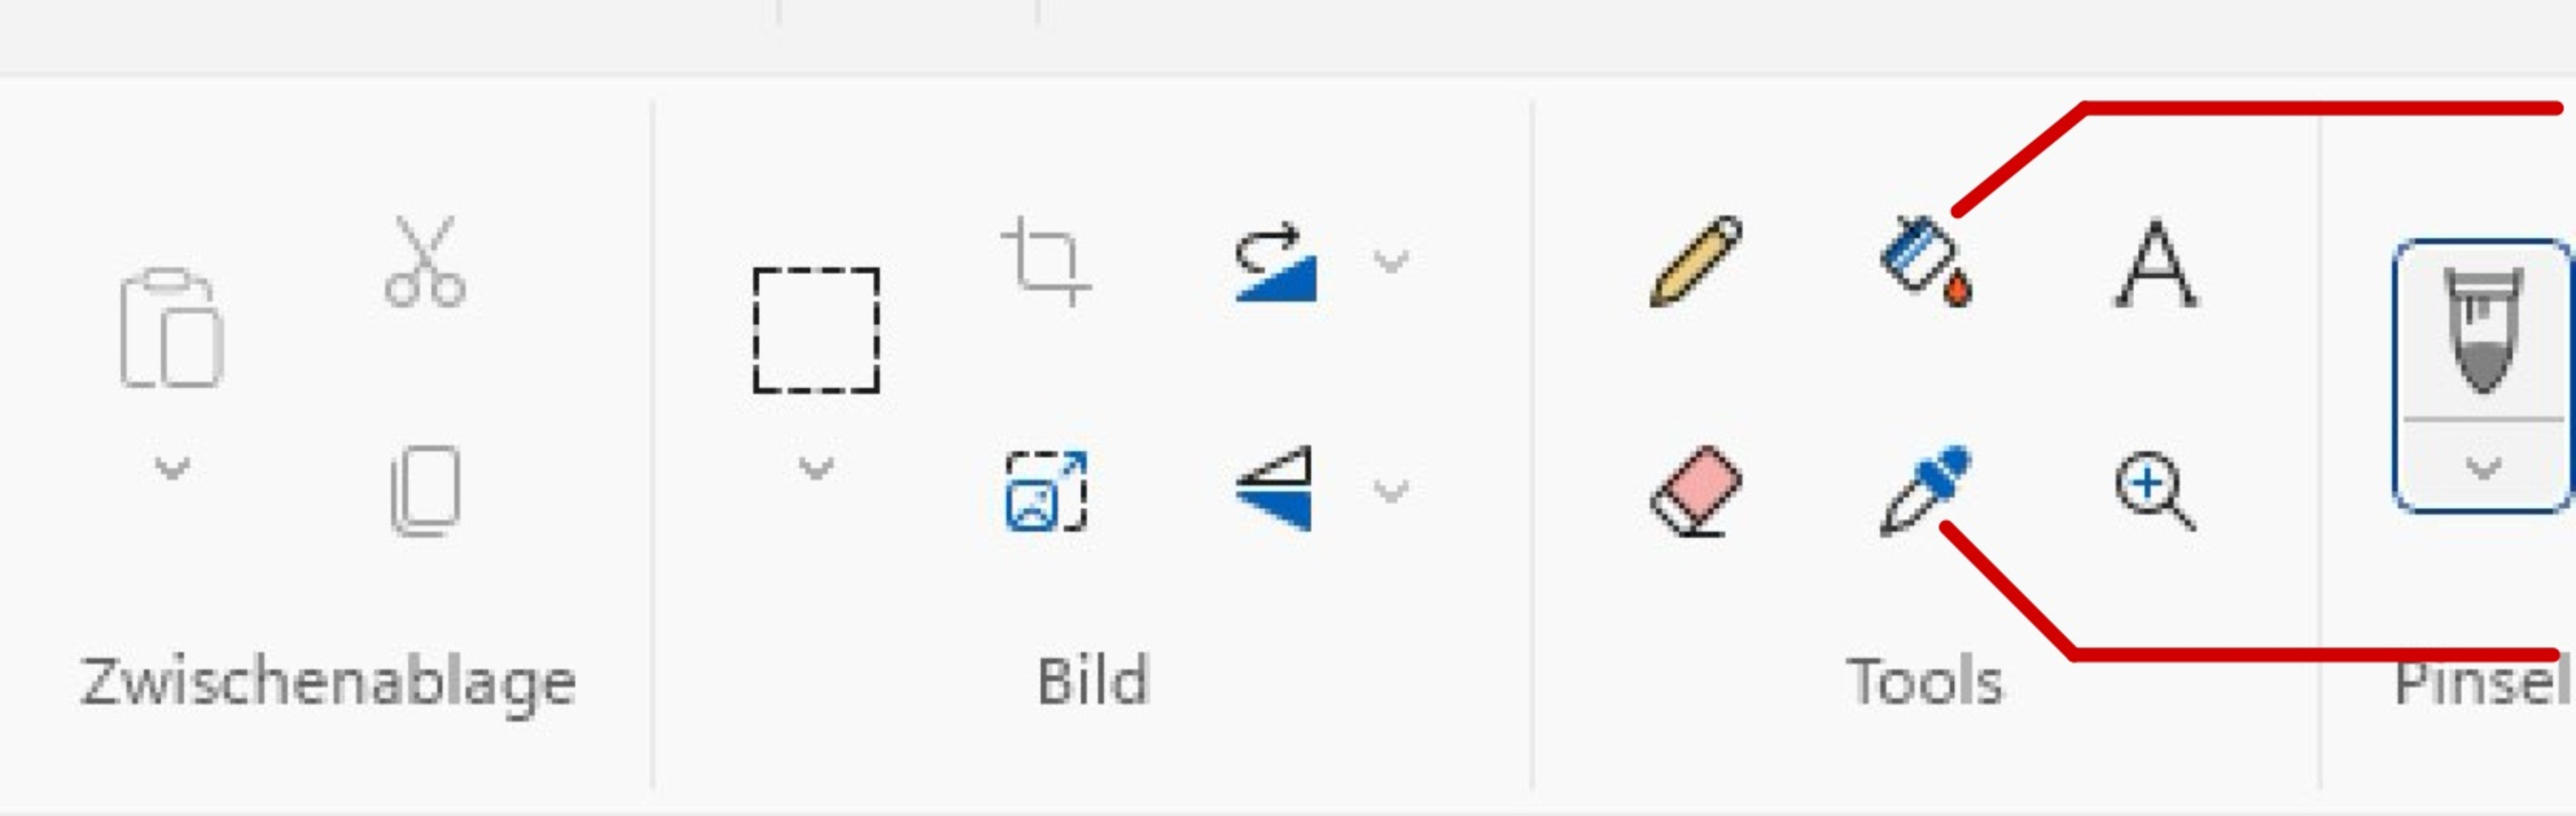
\includegraphics[width=\linewidth]{Paint.pdf}
	\end{minipage}
	\hfill
	\begin{minipage}{0.39\textwidth}\vspace{0pt}
			\textbf{Der Fülleimer} gießt eine ausgewählte Farbe in ein Feld, welches lückenlos von einer anderen Farbe umschlossen wird.\\
			
			\textbf{Der Farbwähler} nimmt die Farbe des angeklickten Pixels an.
	\end{minipage}
	\begin{minipage}{0.6\textwidth}
	\vspace{0.2cm}
		\begin{itemize}\setlength\itemsep{0pt}
			\item Wähle den Farbwähler aus.
			\item Klicke mit der Maus im ersten Feld des Vogelbildes auf die aussagekräftigste Farbe für diesen Bereich.
			\item Wähle den Fülleimer aus.
			\item Klicke mit der Maustaste auf das erste Feld des weißen Bildes.
			\item Wiederhole dieses Vorgehen für alle neun Felder.
			\item Speichere das fertige Bild in deinem Ordner.
		\end{itemize}
	\end{minipage}
	\begin{minipage}{0.4\textwidth}
		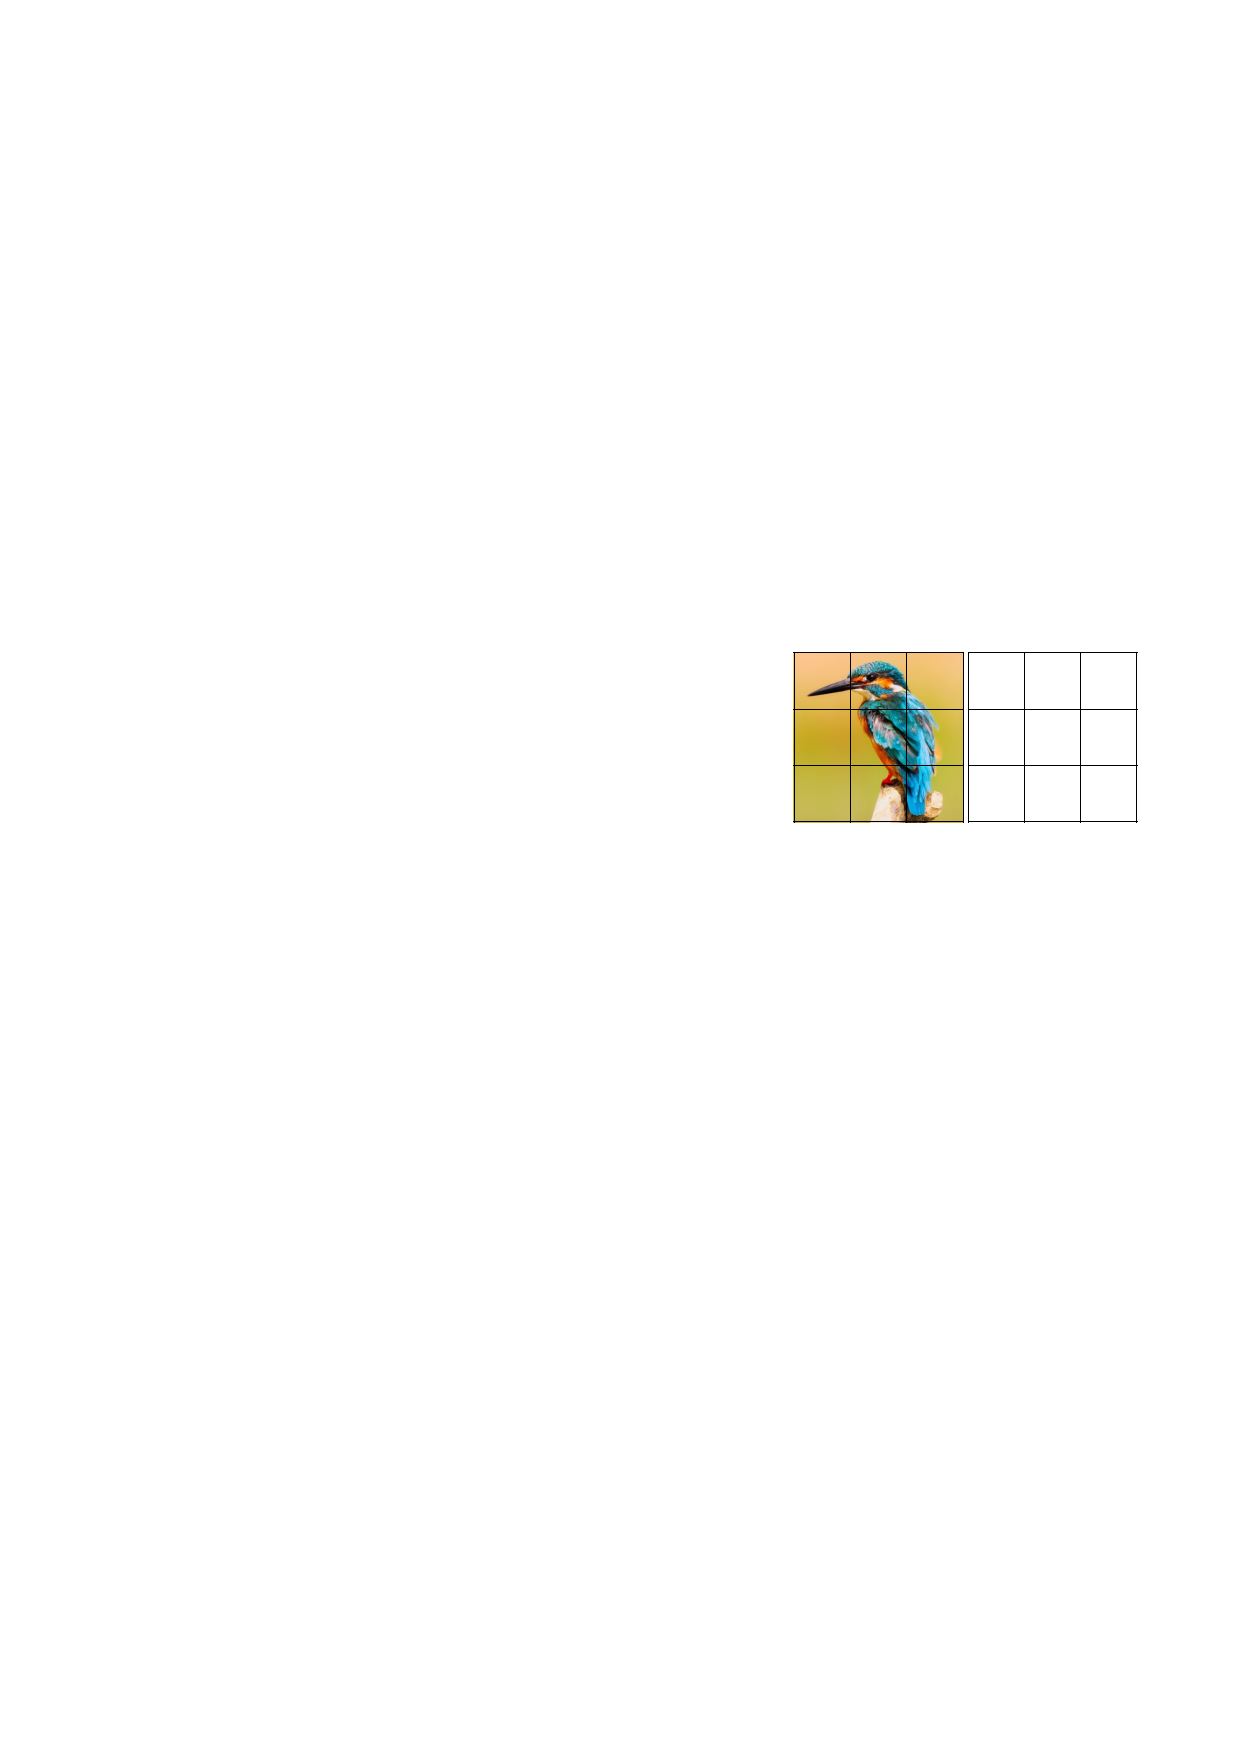
\includegraphics[width=\linewidth]{Vogel3.pdf}
	\end{minipage}

\aufgabe{}
\begin{tasks}
	\task Bewerte die Qualität deines erstellten 3x3 Rasters. Ist der Vogel darauf zu erkennen?
		\liniert{2}
	\task Formuliere einen Lösungsvorschlag zur Verbesserung der Qualität.
		\liniert{2}
\end{tasks}

\aufgabe{}
\begin{minipage}{0.6\textwidth}
		Öffne das Bild "Qualitätsraster 12x12" mit Paint. Bewerte deinen Lösungsvorschlag aus Aufgabe 2b. Formuliere bei Bedarf einen neuen Lösungsvorschlag.\\
		\liniert{2}
	\end{minipage}
	\begin{minipage}{0.4\textwidth}
		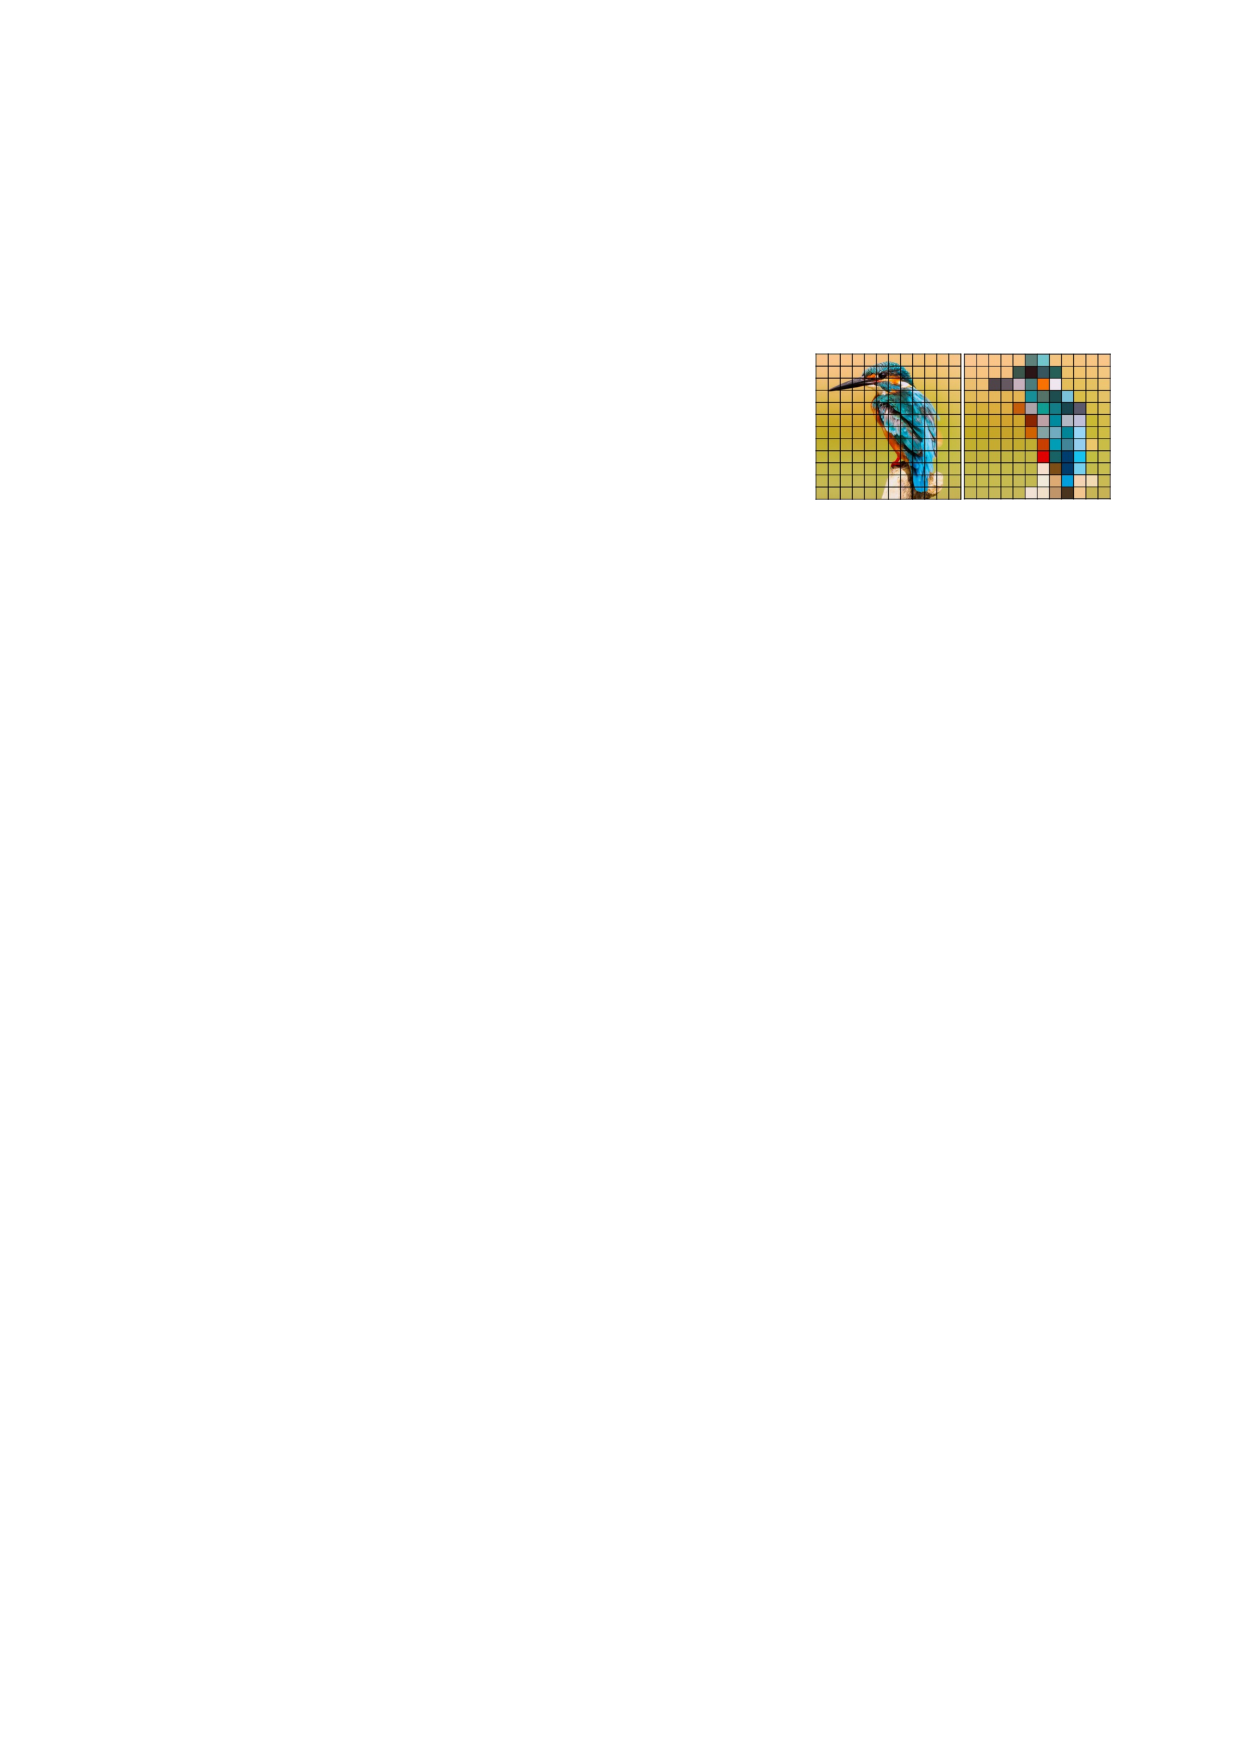
\includegraphics[width=\linewidth]{Vogel12.pdf}
	\end{minipage}
	\vspace{0.2cm}
	\liniert{2}

\aufgabe{}
\begin{minipage}{0.75\textwidth}
		\begin{tasks}
			\task Informiere dich über die Auflösung des Originalbildes "Vogel".\\
			\textit{Tipp: Rechtsklick auf die Datei }$\rightarrow$\textit{ Eigenschaften }$\rightarrow$\textit{ Details}\\
			$\rightarrow$ Die Auflösung beträgt \rule{1.5cm}{0.4pt} Pixel in der Breite und \rule{1.5cm}{0.4pt} Pixel in der Höhe.
			\task Informiere dich über die Auflösung des Displays mit dem du arbeitest.\\
			\textit{Tipp: Suche in dem Betriebssystem die Anzeigeeinstellungen.}\\
			$\rightarrow$ Die Auflösung des Displays beträgt \rule{1.5cm}{0.4pt} Pixel in der Breite und \rule{1.5cm}{0.4pt} Pixel in der Höhe.
			\end{tasks}
	\end{minipage}
	\begin{minipage}{0.25\textwidth}
		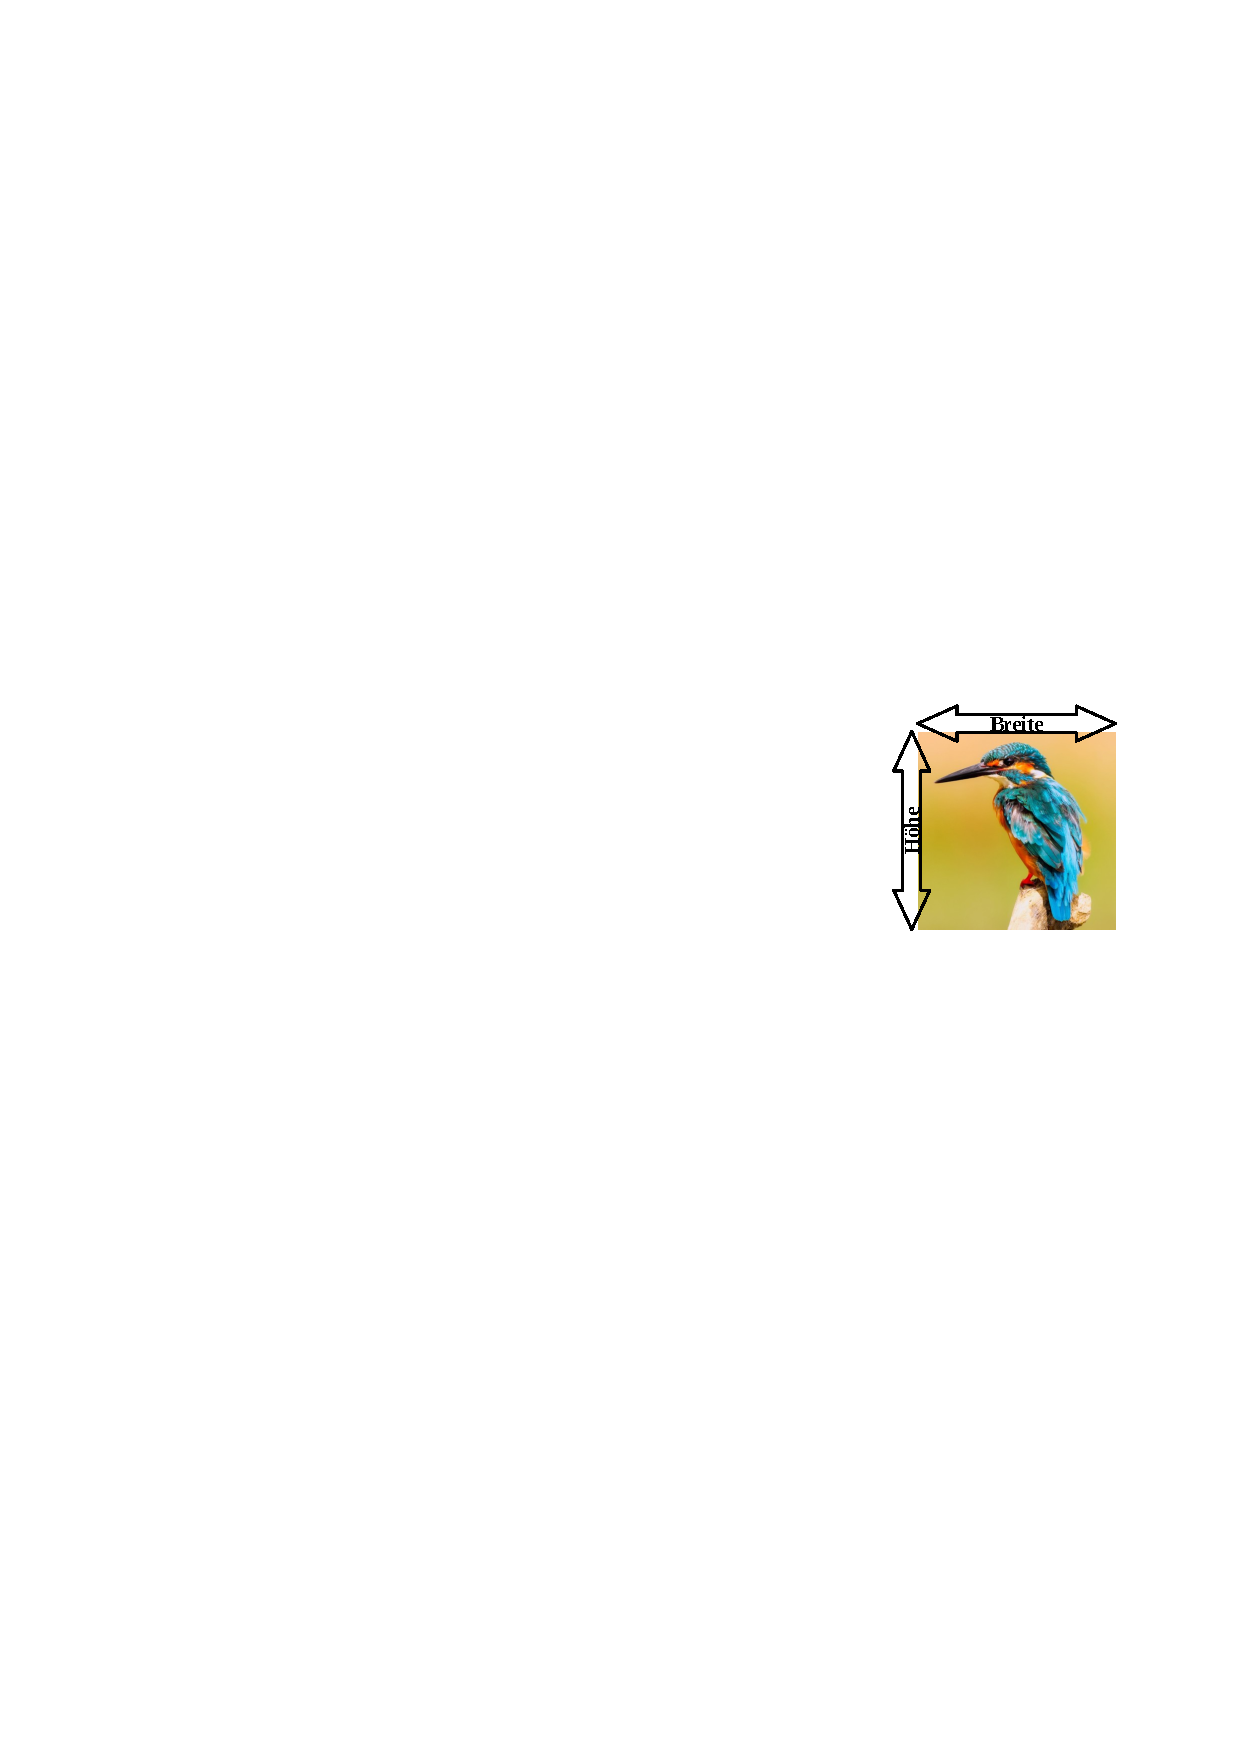
\includegraphics[width=\linewidth]{VogelPixel.pdf}
	\end{minipage}

\aufgabe{}
\begin{minipage}{1\textwidth}
	Vergleiche die beiden Bilder des Spiels Donkey Kong von 1981 und von 2018. Begründe die Qualitätsunterschiede.
\end{minipage}
	\begin{minipage}{0.6\textwidth}
		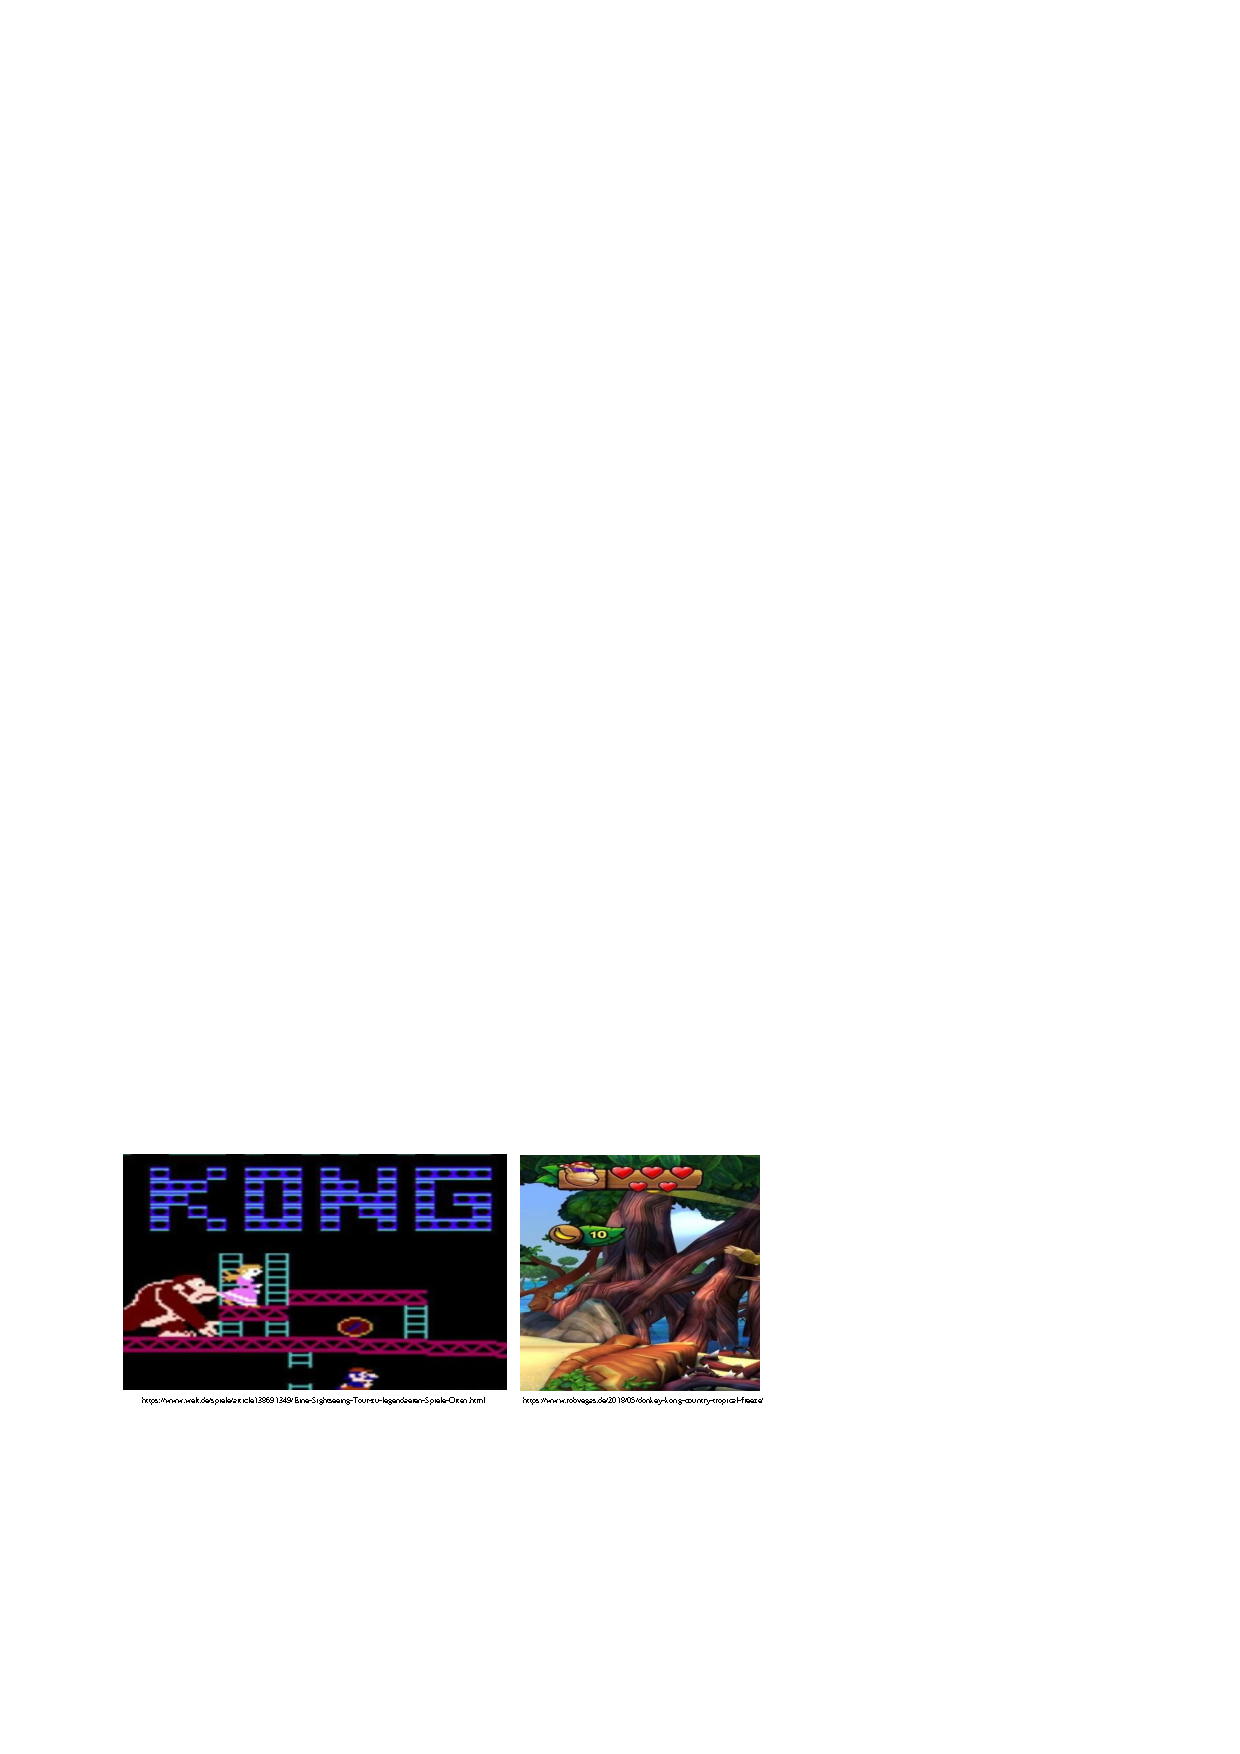
\includegraphics[width=\linewidth]{DonkeyKong.pdf}
	\end{minipage}
	\begin{minipage}{0.4\textwidth}
		\liniert{4}
	\end{minipage}

%\input
\label{LastPage}
\normalsize
\ifthenelse{\equal{\TYP}{Klassenarbeit}}{
\input{\patha/Erwartungsbild.tex}}
{}
\ifthenelse{\equal{\TYP}{Leistungskontrolle}}{
\input{\patha/Erwartungsbild.tex}}
{}


\end{document}